%!TEX root = ../thesis.tex
%*******************************************************************************
%*********************************** VoI demos chapter *****************************
%*******************************************************************************

% keep the discussion of the practical importance of VoI in here, as there's not so much in the methodology chapter
% e.g. VoI allows us to rationalise and prioritise expenditure on data collection

\chapter[Applying \glsxtrshort{voi} to energy systems]{Applying \glsxtrshort{voi} to\\energy systems} \label{chap:demonstrations}

\graphicspath{{Demonstrations/Figs/}}

\begin{cbox}{}
    \printpublication{langtry2024RationalisingDataCollection}

    \noindent{\color{black!50}\rule{\textwidth}{0.4mm}}\vspace{2mm}

    \noindent
    This chapter has been published as the journal article above, as well as a corresponding conference paper \citep{langtry2023ValueInformationAnalysis}.
    The example decision problems in this chapter were developed in collaboration with the co-authors of the article, who are experts on the different energy systems studied. They contributed to the development of the energy system models for each example, and provided a small amount of the text describing those models that appears in this chapter. Other than these contributions, all of the code, analysis, and text in this chapter is my own work.
\end{cbox}

\begin{cbox}{}
    All code and data used to perform the experiments in this chapter is available at \url{https://github.com/EECi/VOI-for-Building-Energy}.
\end{cbox}\

%\newpage

% Brief intro to chapter explaining contents and flow.
\noindent
Having introduced the \glsxtrshort{voi} methodology and how it works in the previous chapter, this chapter demonstrates how \glsxtrshort{voi} can be used to understand data collection requirements in building energy systems. It explores three example decision problems in building energy systems: air source heat pump maintenance scheduling, ventilation scheduling for indoor air quality, and ground-source heat pump system design. In each a different aspect of how \glsxtrshort{voi} can be used to support decision making is illustrated. The examples show how \glsxtrshort{voi} can be used prioritise, rationalise, and justify expenditure on data collection in building energy systems, and avoid wastage on low insight data.\\


%********************************** Intro section **************************************
\section{Introduction}

As explored in the \nameref{chap:introduction}, data can be collected to support decision making in the design and operation of building energy systems by reducing uncertainties, allowing more informed and effective decisions to be taken \citep{molina-solana2017DataScienceBuilding}.
However, data collection is costly.
The cost of data collection must be weighed against the benefits it provides to decision making to determine whether it is economically worthwhile.

Accounting for uncertainties during planning and the use of data collection to support decision making has been standard in the building energy systems field for some time \citep{tian2018ReviewUncertaintyAnalysis,rysanek2013OptimumBuildingEnergy,mavromatidis2018ReviewUncertaintyCharacterisation,mobaraki2022NovelDataAcquisition}.
However, few studies that recommend collecting data discuss its cost. Studies that do quantify data collection costs frequently report only the sensor cost \citep{han2020EnergysavingBuildingSystem,zhai2020AssessingImplicationsSubmetering}, omitting several components of the overall cost of data collection, such as the costs of digital infrastructure, data processing, maintenance, and quality assurance.
Very few studies in the building energy literature have examined the economic benefit of data collection, and quantified the value provided by data collection.
There may exist significant unidentified wastage in building systems in the form of low insight monitoring. This wastage will likely grow if data collection strategies are not rationalised as building digitisation continues to expand.

\newpage
The \glsxtrshort{voi} framework introduced in \Cref{chap:methodology} provides a principled, numerical methodology for quantifying the value of data collection in building energy systems. This allows expenditure on data collection and monitoring systems to be justified, prioritised, and rationalised, and for cost optimal data collection strategies to be determined. So far, no study has used \glsxtrshort{voi} to quantify the benefit that uncertainty reduction from \textit{practical} data collection would provide to decision making in building energy systems.\\

This chapter demonstrates how the \glsxtrshort{voi} methodology can be used to investigate data collection requirements for building energy systems. It presents three example decision problems:
\begin{itemize}
    \item Smart meters to support maintenance scheduling for \glsxtrlong{ashp}s
    \item Occupancy monitoring systems to support ventilation scheduling for indoor air quality in offices
    \item Ground thermal testing to support the design of \glsxtrlong{gshp} based heating systems for apartment blocks
\end{itemize}
Each showing a different decision making context: management, operation, and design respectively.

In each example, \glsxtrshort{voi} is used to study how data collection can improve decision making, and the insights that it can provide are discussed. The examples illustrate different aspects of \glsxtrshort{voi}: representation of complex systems, sensitivity to model assumptions, and determination of optimal measurement precision.

\Cref{sec:ashp,sec:vent,sec:gshp} present the three example decision problems in turn. In each section, the model of the decision problem is described, \glsxtrshort{voi} analysis is performed to study a different aspect of the benefit of data collection, and the insights it provides into the usefulness of that data are discussed. Finally, conclusions are drawn in Section \ref{sec:demonstrations-conclusions}.


\newpage
%********************************** Example problem sections **************************************
%% NOTE: the example problems sections are unchanged from the paper

%%% ASHP %%%
\section[\glsxtrshort{ashp} maintenance scheduling]{Condition measurement for optimising maintenance scheduling for air source heat pumps} \label{sec:ashp}

\glsxtrlong{ashp}s (\glsxtrshort{ashp}s) provide significant advantages to decarbonising the heating of buildings through their ability to exploit ambient heat in the environment to achieve high Coefficients of Performance (\glsxtrshort{cop}s), reducing the direct energy input required to heat a space, and so reducing the embodied carbon emissions of heating. However, through usage, the performance of \glsxtrshort{ashp}s degrades, reducing the \glsxtrshort{cop}s they can achieve. Maintenance activities can be undertaken to address this performance degradation and improve the \glsxtrshort{cop}s achieved by the heat pumps, reducing the electricity consumed and operational costs. However, regular maintenance is costly.

When deciding how frequently to maintain \glsxtrshort{ashp} units, asset owners seek to trade-off the cost of maintenance activities with the benefits they provide in reduced electricity consumption cost to minimise the total cost of operating the \glsxtrshort{ashp} asset. However, the performance of degrading \glsxtrshort{ashp}s depends on several uncertain factors, including the degradation rate, the base Seasonal Performance Factor (SPF), and the performance improvement provided by maintenance. Additionally, at the time maintenance is scheduled, the cost of electricity and the heating load of the building are unknown. Therefore, the maintenance scheduling decision must be made under these uncertainties.

Smart meter data can be used to better estimate the performance of \glsxtrshort{ashp} units, allowing for the scheduling of maintenance to be optimised. However, installing and maintaining smart meters adds additional cost to the operation of the \glsxtrshort{ashp} units. Therefore, asset owners will raise the question, ``Does installing a smart meter on an \glsxtrshort{ashp} unit reduce the overall operating costs by allowing for optimised maintenance scheduling?''.\\

A case involving a research building at the University of Cambridge, which is equipped with 30 identical \glsxtrshort{ashp} units, is examined to assess the economic viability of installing a centralised electricity smart meter to assist maintenance scheduling optimisation. The asset owner selects the number of evenly spaced maintenance activities undertaken per year, $N_m \in \{0,\ldots,12\}$, as to minimise the expected operating cost of the heating system (Eq. \ref{eq:ASHP-total-cost}).\\

\noindent
The annual energy consumed by the \glsxtrshort{ashp} units is given by,
\begin{equation}
    E = \frac{L_H}{\text{SPF}}
\end{equation}
where $L_H$ is the heating load of the building for the coming year. This heating load is assumed to be Gaussian distributed, with mean and standard deviation determined from historic building metering data,
\begin{equation}
    L_H \sim \mathcal{N}\left( L_H, \mu=12.6, \sigma=1.36 \right) \:\: \text{GWh/year}
\end{equation}

\noindent
The total cost of electricity consumed to meet the building heating load is given by,
\begin{equation}
    C_e = p_e E
\end{equation}
where $p_e$ is the price of electricity for the coming year, which is assumed Gaussian with mean and standard deviation calculated using consumer electricity cost data across UK regions from 2022 \citep{desnz2023AnnualDomesticEnergy},
\begin{equation}
    p_e \sim \mathcal{N}\left( p_e, \mu=32.6, \sigma=1.6 \right) \:\: \text{p/kWh}
\end{equation}

\noindent
The annual Seasonal Performance Factor ($\text{SPF}$) of the \glsxtrshort{ashp}s, the average \glsxtrshort{cop} over the heating season, is given by,
\begin{equation}
    \text{SPF} = \text{SPF}'(1-\alpha)(1+\beta)
\end{equation}
where $\text{SPF}'$ is the base heat pump SPF, which is not known at the time of installation. Using data from existing \glsxtrshort{ashp} units \citep{nouvel2015EuropeanMappingSeasonal}, it is assumed to be distributed as,
\begin{equation}
    \text{SPF}' \sim \mathcal{N}\left( \text{SPF}', \mu=2.9, \sigma=0.167 \right)
\end{equation}
$\alpha$ is the performance degradation factor of the \glsxtrshort{ashp}s, which is modelled as being distributed as a truncated Normal with mean 0.01 and standard deviation 0.25, as it is a non-negative parameter,
\begin{equation}
    \alpha \sim \mathcal{N}(\alpha, \mu=1e{-}2,\sigma=0.25 : \alpha \geq 0)
\end{equation}
$\beta$ models the performance improvement provided by maintenance activities, and is given by,
\begin{equation}
    \beta = \frac{\beta_a N_m^\gamma}{\beta_b + N_m^\gamma} (1+\varepsilon)
\end{equation}
the parameters $\beta_a$, $\beta_b$, $\gamma$, are empirical parameters with assumed values of 0.05, 2.5, and 1.4 respectively \citep{griffith2008MethodologyModelingBuilding}. The parameter $\varepsilon$ models uncertainty in the performance improvement, and is taken to be distributed as,
\begin{equation}
    \varepsilon \sim \mathcal{N}(\varepsilon, \mu=0,\sigma=0.1)
\end{equation}
The cost per activity of performing maintenance on all 30 \glsxtrshort{ashp} units, $C_m$, is taken to be £18,000 \citep{daikin2022DaikinUKPrice}. So, the total cost of operating the \glsxtrshort{ashp}s (comprised of electricity and maintenance costs) is given by,
\begin{equation} \label{eq:ASHP-total-cost}
    C_{\text{total}} = C_e + C_m N_m
\end{equation}

The described stochastic decision problem of optimally scheduling \glsxtrshort{ashp} maintenance is represented in influence diagram form in Fig. \ref{fig:ID-ASHP-maintenance}, where grey arrows represent measurements. This diagrammatic representation provides a far clearer, more concise, and readily extendable description of the decision task within this complex engineering system.\\

\begin{figure}[h]
    \centering
    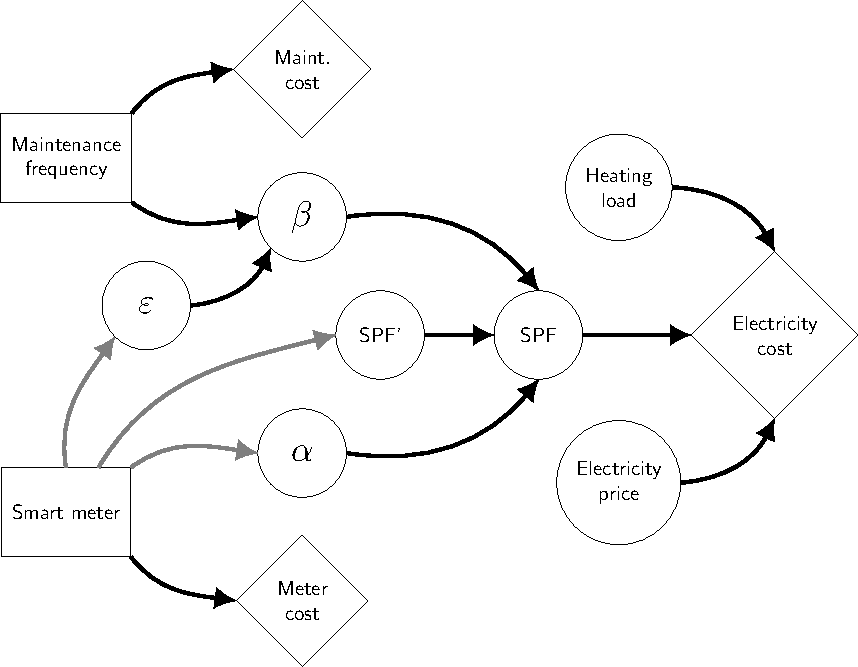
\includegraphics[width=0.75\linewidth]{ASHP-ID.pdf}
    \vspace{2pt}
    \caption{Influence diagram representation of \glsxtrshort{ashp} maintenance scheduling decision problem}
    \label{fig:ID-ASHP-maintenance}
\end{figure}

\newpage
Solving the Prior decision problem\footnote{\label{fn:pdp-defn} Refer back to \Cref{sec:methodology-bayesian-decision-analysis} for definition.}, the optimal maintenance frequency is found to be 2 activities per year, leading to an expected operating cost (Eq. \ref{eq:ASHP-total-cost}) of £1,876,300/year for the building heating system, of which £36,000/year (2\%) is spent on maintenance. Fig. \ref{fig:ASHP-prior-dist} plots the probability distribution of operational costs for the system when maintained 2 times a year. It demonstrates the significance of the uncertainties in the building energy system on the planning problem, as the cost of operating the heating system can vary from £1m/year to £4m/year, and so highlights the importance of accounting for those uncertainties during planning.

Solving the Pre-Posterior decision problem\footnoteref{fn:pdp-defn} with perfect information, i.e. planning maintenance with perfect knowledge of the uncertain parameters in the system, achieves an expected cost of £1,874,640/year. Therefore the Expected Value of Perfect Information (\glsxtrshort{evpi}), as defined in \Cref{sec:methodology-voi}, is £1,660/year.

Fig. \ref{fig:ASHP-post-action-freqs} shows the distribution of optimal maintenance frequency when the true values of the uncertain system parameters are known. In slightly over half of cases, perfect information about the system does not change the maintenance scheduling decision, i.e. the true solution is the same as the prior solution, indicated by the black column. However the information provides value, as in many cases the performance degradation of the \glsxtrshort{ashp}s is less severe, with less frequent maintenance providing lower operational cost. Monitoring information allows the system operator to avoid the cost of unnecessary maintenance activities in these cases.\\

\begin{figure}[h]
    \centering
    \begin{minipage}{.475\textwidth}
        \centering
        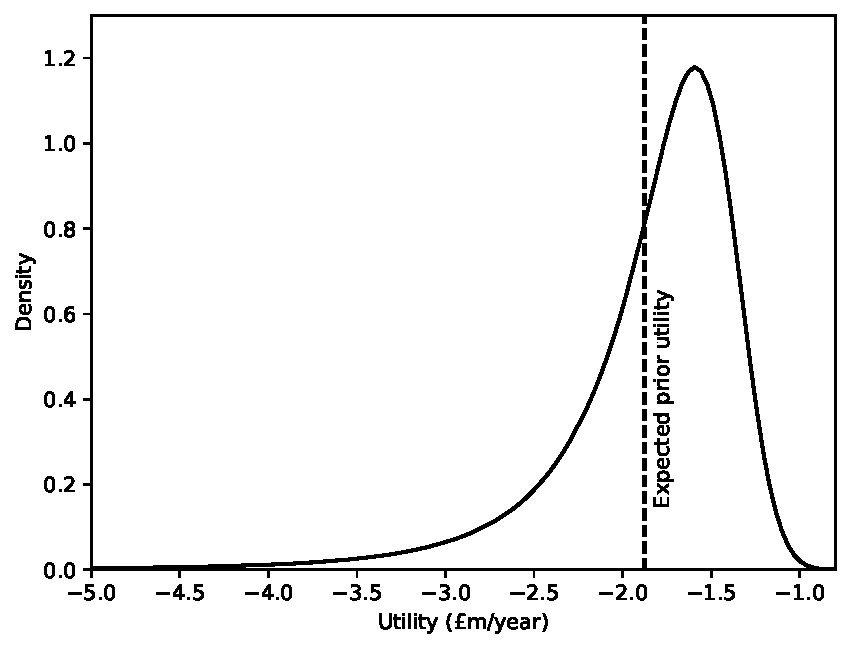
\includegraphics[width=\linewidth]{ASHP_prior_utility_distribution.pdf}
        \caption{Distribution of utilities achieved by optimal prior action, ${N_m}^*=2$. Dashed line indicates mean of distribution}
        \label{fig:ASHP-prior-dist}
    \end{minipage}%
    \hfill
    \begin{minipage}{.475\textwidth}
        \centering
        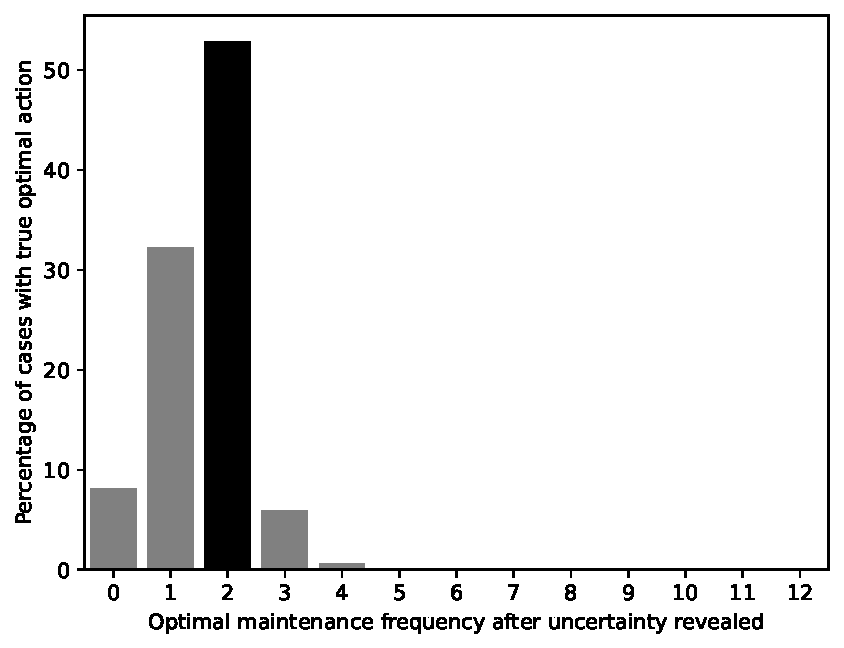
\includegraphics[width=\linewidth]{ASHP_posterior_action_freqs.pdf}
        \caption{Distribution of true optimal maintenance frequency, i.e. best action once uncertainty has been revealed}
    \label{fig:ASHP-post-action-freqs}
    \end{minipage}%
\end{figure}

\newpage
The annualised cost of the electricity smart meter used to monitor the \glsxtrshort{ashp} units (`meter cost' in Fig. \ref{fig:ID-ASHP-maintenance}) is estimated to be £70/year \citep{daikin2022DaikinUKPrice}. Therefore, the installation of smart meters capable of perfectly measuring \glsxtrshort{ashp} performance, degradation, and building load, and the dynamic scheduling of maintenance activities using the actual electricity price, would lead to a net economic benefit, \glsxtrshort{voi} minus information cost, of £1,590/year to the asset owner from reduced operational costs. In this way, the asset owner can justify their investment in smart meters.
% Or, conclude that: 1. this is very small c.f. the total operational cost, 2. true VoI is smaller, 3. this is only hardware cost (?) - so overall, probably not worth installing smart meters
The value of information provided by smart meters in this scenario is small compared to the total operational costs, only 0.06\%. However, the use of smart meters to optimise maintenance scheduling can provide additional benefits, such as extending the lifespan of the \glsxtrshort{ashp} units and decreasing the probability of malfunctions. These cost savings, although not accounted for in these calculations due to simplification, could be significant.\\


%%% Ventilation %%%
\section[Office ventilation scheduling]{Building occupancy measurement for real-time ventilation scheduling to improve indoor air quality} \label{sec:vent}

In mechanically ventilated office spaces, building managers must schedule ventilation system settings to ensure sufficient indoor air quality for the occupants. Adequate ventilation is required to prevent the transmission of airborne infectious diseases such as the SARS-CoV-2 virus (COVID-19), which is both damaging to the health of the occupants and costly for the tenant of the office space through lost productivity. However, operating ventilation at an unnecessarily high rate can impact occupant thermal comfort, lead to excessive carbon emissions, as well as excessive operational cost of the ventilation system through the additional heating/cooling demand required to condition air intake. The risk of viral transmission, and thus the appropriate ventilation setting, is highly dependent on the number of occupants in the office space. However, in the absence of occupant monitoring and dynamic ventilation control systems, building managers must schedule ventilation system settings without knowledge of the exact occupancy level of the space. At the time of deciding ventilation scheduling, the occupancy of the ventilated space over the operation period is uncertain. This uncertainty is particularly relevant in light of recent trends towards `work from home', which reduces the predictability of office occupancy.

This raises the question, ``Would it be worth installing a smart occupancy monitoring and ventilation control system in an office space to improve ventilation scheduling?'', i.e. would the economic benefit of improved ventilation control be greater than the cost of installing such a smart monitoring and control system?\\

A simple model of indoor air quality in a typical office space is considered. Said office space is taken to have a maximum occupancy of 100 people, a floor area of 1,000 m$^2$, and a ceiling height of 2.4 m. There are five available ventilation settings: 1, 3, 6, 12, and 20 air changes per hour (ACH). The ventilation system is assumed to have a fan of specific power 1.9 W/l/s, $P_{\text{fan}}$, operating at 60\% efficiency, $\eta$, for 10 hours per day, $T$. At an electricity unit price of 32.6 p/kWh, $p_e$, the cost of operating the ventilation system\footnote{The cost of heating/cooling associated with ventilation is neglected for simplicity, but can be readily added to the model.} at each setting is calculated as,
\begin{equation}
    C_{\text{vent}} = \text{ACH} \times V \times \frac{P_{\text{fan}}}{\eta} \times T \times p_e
\end{equation}
where $V$ is the volume of the office in litres, $T$ is expressed in seconds and $p_e$ in £/Wh.

A model of the probability of viral infection for an individual in an indoor space as described in \citep{deoliveira2021EvolutionSprayAerosol} is used, which is also available in web application form at \href{https://airborne.cam/}{\nolinkurl{airborne.cam}} \citep{gkantonas2021AirborneCamRisk}. It is assumed that the base prevalence of infection amongst the occupants is that of the general UK population in February of 2023, 2.18\% \citep{ons2023CoronavirusCOVID19Latest}, and that infection of an individual leads to 3 days of sick leave, which taking the median daily salary for full-time employees in 2022, costs the tenant £128/day \citep{ons2022EmployeeEarningsUK} in lost productivity.
It is further assumed that any occupants are present in the office space for the whole 8 hour work day, that time coupling effects between days can be neglected, i.e. that the model for a single day is representative, and so illness costs are calculated using the expected number of infections for the given occupancy. The prior distribution of occupancy is taken to be discrete uniform in the interval 0 to 100 inclusive.

The stochastic decision problem is thus to select the ventilation system setting which minimises the sum of the ventilation system operation (electricity) cost, and the cost of lost productivity due to illness to the tenant, subject to uncertainty in the occupancy level of the space.
\begin{equation}
    C_{\text{total}} = C_{\text{vent}}(\text{ACH}) + n \times p_{\text{infection}}(n,\text{ACH})
\end{equation}
where $n$ is the number of occupants in the office.

This decision problem can be described via the influence diagram provided in Fig. \ref{fig:ID-building-vent}.\\

\begin{figure}[p]
    \centering
    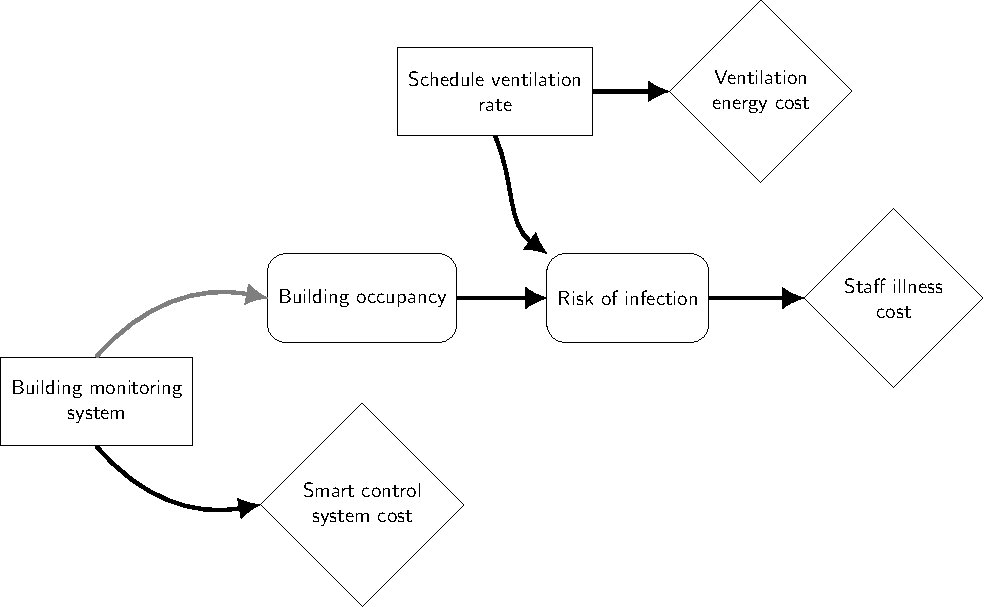
\includegraphics[width=0.66\linewidth]{building-vent-ID.pdf}
    \vspace{4pt}
    \caption{Influence diagram representation of building ventilation scheduling decision problem} \label{fig:ID-building-vent}
\end{figure}

\begin{figure}[p]
    \centering
    \begin{minipage}{.475\textwidth}
        \centering
        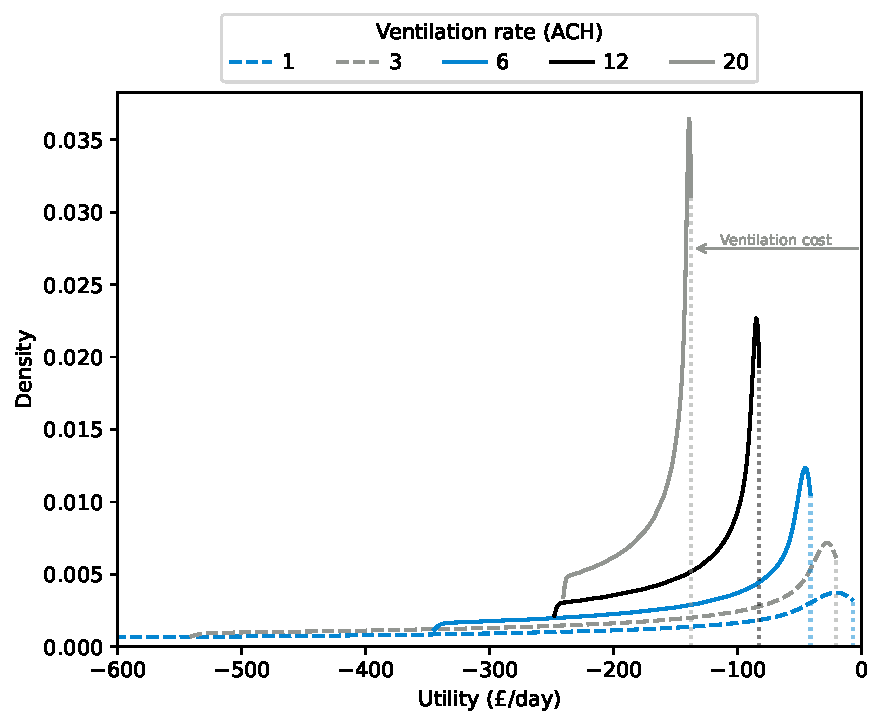
\includegraphics[width=0.975\linewidth]{building_vent_prior_u_dists_by_action.pdf}
        \caption{Distribution of utilities achieved by each ventilation rate under prior uncertainty}
        \label{fig:b_vent_a_dists}
    \end{minipage}%
    \hfill
    \begin{minipage}{.475\textwidth}
        \centering
        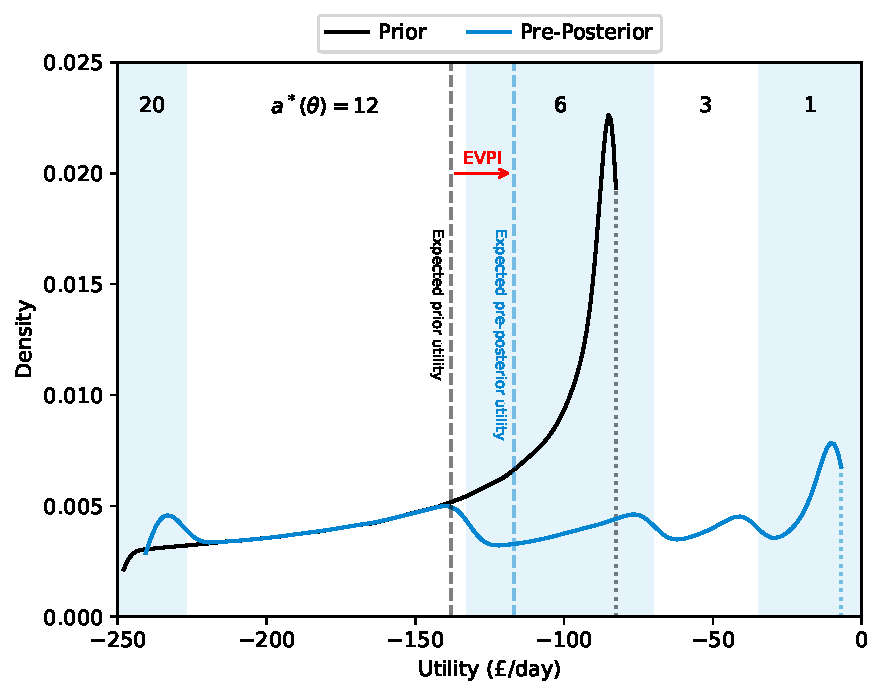
\includegraphics[width=0.95\linewidth]{building_vent_dists_prior_vs_pre_post.pdf}
        \caption{Distribution of utilities achieved by prior and pre-posterior decisions}
    \label{fig:b_vent_prior_vs_prepost}
    \end{minipage}%
\end{figure}

\begin{figure}[p]
    \centering
    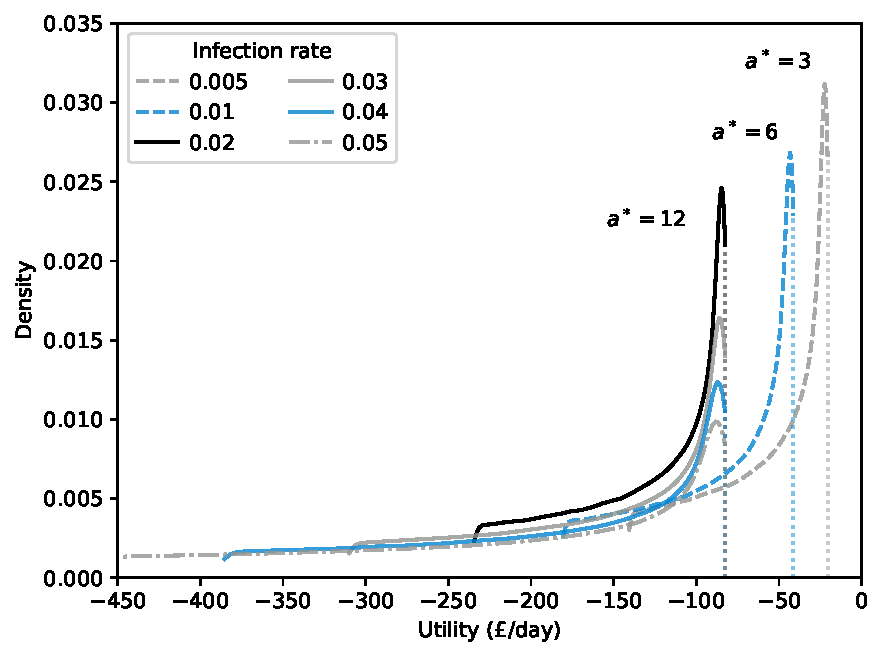
\includegraphics[width=0.45\linewidth]{building_vent_prior_u_dists_with_InfRate.pdf}
    \caption{Distributions of utilities for prior solution with varying assumed infection rate} \label{fig:b_vent_sensitivity}
\end{figure}

Solving the Prior decision problem, the optimal ventilation rate is found to be 12 air changes per hour, leading to an expected overall cost of £138/day for the tenant. Fig. \ref{fig:b_vent_a_dists} shows the distribution of utilities for each available ventilation rate under the prior uncertainty. Increasing the ventilation rate increases the base cost of all outcomes, indicated by the dashed line showing the minimum cost for each curve, but reduces the risk of large numbers of infections occurring when the office has high occupancy, limiting the maximum cost. The utility distribution for the prior optimal ventilation rate of 12 ACH in the base case is indicated by the black curve in Figures \ref{fig:b_vent_a_dists} to \ref{fig:b_vent_sensitivity}.
% discuss risk vs mean reward trade-off??

Solving the Pre-Posterior decision problem with perfect information, i.e. dynamically scheduling ventilation with perfect knowledge of occupancy from a monitoring system, achieves an expected cost of £117/day. Therefore, the \glsxtrshort{evpi} is £21/day. Hence, over a 20 year operational lifetime, the smart monitoring and control system could save the tenant up to £850,000, or 15\% of the total operating cost. Fig. \ref{fig:b_vent_prior_vs_prepost} plots the distribution of utilities achieved by the prior and pre-posterior decisions. For the prior, the same decision of 12 ACH is used in all cases as no measurement is taken. Whereas, for the pre-posterior, the ventilation rate is set using information on the occupancy level in each case. The blue regions indicate the regime of cases where each ventilation rate is selected by the pre-posterior decision, i.e. where it is the lowest cost choice. The pre-posterior density is similar to the prior in the region of high costs, but is much more uniform and extends substantially further into the low cost region, indicating that the \glsxtrshort{voi} is primarily derived from the ability to reduce ventilation rate and save electricity cost when office occupancy is low.

Building managers can use the computed \glsxtrshort{evpi} to support their decision making about whether investment in smart occupancy monitoring and ventilation control systems are worthwhile. If a proposed smart monitoring and control system is expected to have an installation and maintenance cost over the 20 year lifetime of more than £850,000, then this investment will not be beneficial for the context of ventilation scheduling. A cheaper but less precise method of estimating occupancy, such as a desk booking system, may be a more suitable strategy, or it may be most cost effective to forego occupancy measurement altogether and use a fixed ventilation rate.

%% Sensitivity analysis, discuss implications
\subsection*{Sensitivity analysis}
The problem formulation considered assumes a variety of properties about the office being ventilated. However, commercial building stocks are diverse, and the actual value of these properties varies between buildings. A sensitivity analysis is performed to investigate whether occupancy monitoring and dynamic ventilation scheduling remains valuable across different sized offices. The \glsxtrshort{voi} analysis is repeated for office models with 5 to 25 m$^2$ of floor area per person, maintaining a maximum occupancy of 100, and keeping all other properties as before. Table \ref{tab:floor-area-sensitivity} provides the optimal ventilation rate without measurement and the \glsxtrshort{evpi} for each size of office considered. The \glsxtrshort{evpi} is lowest in the extreme cases where extreme ventilation rates are optimal both on average (for the prior problem) for the majority of occupancy outcomes. For instance, in the smallest office, the highest available ventilation rate of 20 ACH is the optimal prior decision, and the optimal decision for 53\% of occupancy outcomes. For all office sizes tested, the \glsxtrshort{evpi} remains significant, 10\% or more of the prior expected cost, suggesting that occupancy monitoring systems are likely beneficial for offices of any size.\\

\begin{table}[h]
    \centering
    \renewcommand{\arraystretch}{1}
    \begin{tabular}{c|ccccc} \toprule \toprule
        Floor area per person (m$^2$) & \: 5 \: & \: 10 \: & \: 15 \: & \: 20 \: & \: 25 \: \\ \midrule
        Prior optimal ventilation rate (ACH) & 20 & 12 & 6 & 3 & 3 \\
        \glsxtrshort{evpi} (£/day) & 14 & 21 & 16 & 19 & 14 \\
        \bottomrule \bottomrule
    \end{tabular}
    \smallskip
    \caption{Sensitivity of prior solution and \glsxtrshort{evpi} to office size}
    \label{tab:floor-area-sensitivity}
\end{table}

The prevalence of viral illness in the general population has a significant impact on the risk of infection spreading in an office environment, and so should be taken into account by a building manager when setting ventilation rates, and as a result when determining what information is required to support that decision. The sensitivity of the prior decision and \glsxtrshort{evpi} is tested for infection rates from 0.5\% to 5\% \citep{ons2023CoronavirusCOVID19Latest}. Table \ref{tab:inf-rate-sensitivity} provides the results of this analysis, and Fig. \ref{fig:b_vent_sensitivity} plots the distribution of utilities for the prior solutions at each infection rate. As infection rate increases, the risk of infection at a given occupancy level rises, causing a widening of the utility distribution, and so greater risk for the decision maker. Additionally, the distribution of true optimal ventilation rates flattens. Hence, for more occupancy outcomes a different ventilation rate to the prior is optimal, and the benefit of that improved decision increases. Therefore, the greater the infection rate, the higher the \glsxtrshort{voi}, and the more valuable occupancy monitoring becomes. The sharp increase in \glsxtrshort{evpi} between infection rates of 1\% and 2\% highlights the importance of using sensitivity analysis to determine whether conclusions about the economic benefits of data collection derived from \glsxtrshort{voi} analysis remain valid as assumptions about the studied building energy system are varied. Alternatively, assumed parameters can be modelled as uncertainties and included within the system model.\\

\begin{table}[h]
    \centering
    \renewcommand{\arraystretch}{1}
    \begin{tabular}{c|cccccc} \toprule \toprule
        Infection rate (\%) & 0.5 & 1 & 2 & 3 & 4 & 5 \\ \midrule
        Prior optimal ventilation rate (ACH) & 3 & 6 & 12 & 12 & 12 & 12 \\
        \glsxtrshort{evpi} (£/day) & 8 & 11 & 22 & 21 & 24 & 30 \\
        \bottomrule \bottomrule
    \end{tabular}
    \smallskip
    \caption{Sensitivity of prior solution and \glsxtrshort{evpi} to infection prevalence in the population}
    \label{tab:inf-rate-sensitivity}
\end{table}


%%% GSHP %%%
\section[\glsxtrshort{gshp} borehole design]{Ground conductivity measurement for optimising borehole design in residential ground source heat pump heat supply systems} \label{sec:gshp}

\glsxtrlong{gshp} (\glsxtrshort{gshp}) systems use the ground as a source and sink of heat to provide cooling and heating for buildings in a highly energy efficient way \citep{aresti2018ReviewDesignAspects}. As these systems exchange heat with the ground, their performance (characterised by the \glsxtrshort{cop}s they achieve) is influenced significantly by the geological properties of the ground with which they exchange heat. In the design of such \glsxtrshort{gshp} heating \& cooling supply systems, it is desired to match the capacity of the \glsxtrshort{gshp} system to energy demand of the building as to minimise the overall cost of operating the supply system over its lifetime. The overall operating cost is composed of the capital cost of constructing the system, and the operational costs, which are primarily the cost of the electricity required to meet the building energy demands. Under-specification of the systems leads to greater electricity usage from less efficient and so higher cost auxiliary heating systems, whilst over-specification of the system results in unnecessary capital cost.

At the time of system design, the thermal properties of the ground are typically not known precisely, as existing geological survey data provides an uncertain estimate of the ground properties in the site location \citep{dallasanta2020UpdatedGroundThermal}. However, the system designer has the option to commission thermal tests at the site location prior to designing the \glsxtrshort{gshp} system. Whilst these tests reduce the uncertainty in the ground thermal properties, they are time-consuming and incur additional costs. As a result, these tests are often not conducted, and generally available information on materials and location is used to provide uncertain estimates of ground thermal properties which are used to design the \glsxtrshort{gshp} system. This therefore poses the following question to the designer, ``Would commissioning thermal tests reduce the overall lifetime cost of the \glsxtrshort{gshp} heat supply system by improving the matching of the designed system capacity to the building load?''.\\

A simplified \glsxtrshort{gshp} system design task for a residential building heat supply system is considered. In this design task, the designer must select the length of boreholes, $L_{\text{bh}}$, to be drilled for the ground heat exchange. The available length choices are 110 to 190 m, in 5 m increments. The capital cost of borehole drilling is taken to be 70 £/m/borehole.

It is assumed that the effective ground thermal conductivity, $\lambda_{\text{ground}}$, is the only uncertain geological parameter, and that it is Normally distributed with mean 1.94 W/mK, and standard deviation 0.31 W/mK,
\begin{equation}
    \lambda_{\text{ground}} \sim \mathcal{N}(\mu=1.94,\sigma=0.31) \:\: \text{W/mK}
\end{equation}
which is the average thermal conductivity over the range of borehole depths considered, and covers typical uncertainty ranges given the heterogeneity present in soils \citep{busby2018ModellingStudyVariation,busby2011ProvisionThermalProperties,loveridge2013ThermalResponseTesting}.

The designed \glsxtrshort{gshp} system, consisting of 12 boreholes, must supply heat to a small apartment block of 10 flats over a 50 year operational lifetime. The building is assumed to have a typical heating demand distribution for its type, and a simplified load profile is synthesised based on demand values for the UK \citep{mitchell2020UKPassivhausEnergy}, and using historic weather data for London. This synthetic load profile, $E_{\text{load}}(t)$, consumes 116MWh/year, corresponding to a 13.2 kW mean heating load for the building, with a peak load power of 30.5 kW. The data can be found in the \href{https://github.com/EECi/VOI-for-Building-Energy}{GitHub repository}.

The model of geothermal borehole operation presented in \citep{lamarche2007NewContributionFinite} is used to determine the scheduling of energy extracted from the ground in each time instance, $E_g(t)$, with the borehole fluid temperature, $T_{\text{fluid}}$, conservatively constrained to be within the range $5$ degC to $35$ degC,
\begin{equation}
    5 \leq T_{\text{fluid}}(t) \leq 35
\end{equation}
In this model, $T_{\text{fluid}}$ is a function of the power extracted from the ground, $E_g(t)$, the ground thermal conductivity, $\lambda_{\text{ground}}$, the borehole length, $L_{\text{bh}}$, and the other assumed ground condition parameters.

Given the fluid temperature schedule determined, the instantaneous \glsxtrshort{cop} of the \glsxtrshort{gshp} system is computed using the following empirical relationship from \citep{kensa2014HowCOPVaries},
\begin{equation}
    \text{COP}(t) = 4.0279 +0.1319 \cdot T_{\text{fluid}}(t)
\end{equation}
The energy that is provided by the \glsxtrshort{gshp} system to the building is then given by,
\begin{equation}
    E_{\text{GSHP}}(t) = \frac{E_g(t)}{1-1/\text{COP}(t)}
\end{equation}
If the \glsxtrshort{gshp} system is unable to meet the building load in any time instance, the remaining unsatisfied load is provided by an auxiliary heat supply system with a \glsxtrshort{cop} of 1.
\begin{equation}
    E_{\text{load}}(t) = E_{\text{GSHP}}(t) + E_{\text{aux}}(t)
\end{equation}
The total electricity consumption of the combined heat supply system is therefore given by,
\begin{equation}
    e_{\text{total}} = \sum_t \left( \frac{E_{\text{GSHP}}(t)}{\text{COP}(t)} + E_{\text{aux}}(t) \right)
\end{equation}
The cost of electricity used by the residential building is taken to be 32.6 p/kWh.

The stochastic decision problem of designing borehole lengths as to minimise the expected lifetime cost of the heating supply system is represented as an influence diagram in Fig. \ref{fig:ID-GSHP-design}.\\

\begin{figure}[h]
    \centering
    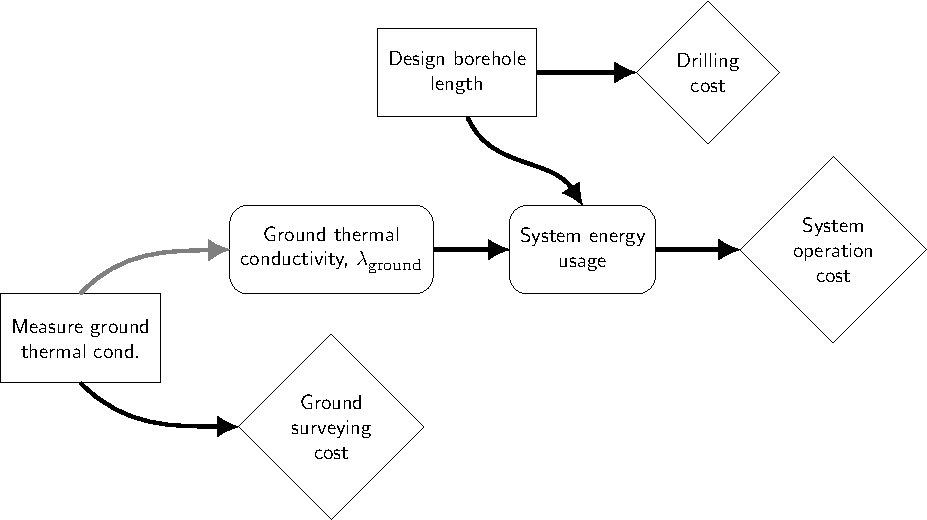
\includegraphics[width=0.8\linewidth]{GSHP-design.pdf}
    \vspace{4pt}
    \caption{Influence diagram representation of \glsxtrshort{gshp} heat supply system design decision problem}
    \label{fig:ID-GSHP-design}
\end{figure}

Solving the Prior decision problem, the optimal borehole length is found to be 155 m, leading to an expected overall lifetime cost of £819,100 for the heating system.

Various technologies exist for measuring ground thermal properties. Table \ref{tab:ground-tests} presents the cost and experimental uncertainty of thermal probe tests and Thermal Response Tests (TRT),  which are commonly used for ground thermal conductivity measurement. The extended TRT measurement is a hypothesised base case for the results achievable with TRT methods. The likelihood of obtaining a measurement $z$ for each test given a true underlying ground thermal conductivity of $\lambda$ is modelled using a Gaussian distribution as,
\begin{equation}
    f_e(z|\lambda) \sim \mathcal{N} \left( z,0,\frac{\nu_e}{2} \lambda \right)
\end{equation}
where $\nu_e$ is the decimal experimental uncertainty of the test.
% Mention that we use Stan to sample from the posterior - as it's quite complicated

\begin{table}[h]
    \centering
    \renewcommand{\arraystretch}{1}
    \begin{tabular}{c|c|c|c} \toprule \toprule
        Method & Uncertainty & Cost (£) & References \\ \midrule
        Thermal probe (in situ) & 25\% & 187 & {\footnotesize \citep{king2012FieldDeterminationShallow}, \citep{sunbeltrentals2023ThermtestTLS100Thermal}} \\
        Thermal probe (lab test) & 17\% & 1,800 & {\footnotesize \citep{low2013MeasuringSoilThermal}, \citep{basaltridgetestinglaboratory2024BasaltRidgeTesting}} \\
        Thermal Response Test (TRT) & 10\% & 5,000 & \makecell{\footnotesize \citep{choi2021DevelopmentChillerattachedApparatus},\\[-.5ex] \footnotesize\citep{spitler2000SituMeasurementGround},\\[-.5ex] \footnotesize\citep{tang2019SensitiveAnalysisEffective}} \\
        Extended TRT & 5\% & 10,000 & -- \\
        \bottomrule \bottomrule
    \end{tabular}
    \smallskip
    \caption{Uncertainty and cost of ground thermal conductivity measurement tests}
    \label{tab:ground-tests}
\end{table}

The \glsxtrlong{evii} (\glsxtrshort{evii}) is computed for each available test, which is compared to the associated cost to determine the net benefit to decision making provided. Fig. \ref{fig:GSHP-EVIIs} plots the results. All tests provide significant net benefit to the heating system design task, indicating that site specific ground thermal testing should be conducted prior to the design of \glsxtrshort{gshp} based heating systems. The TRT provides the greatest net added value to the decision maker, and so using this \glsxtrshort{voi} analysis, the designer of this energy system can justify and optimise their expenditure on ground testing to support their decision making. This demonstrates that additional uncertainty reduction through more data collection or more precise measurement does not always provide sufficient improvements to decision making to warrant its cost.\\

\begin{figure}[h]
    \vspace*{-0.5cm}
    \centering
    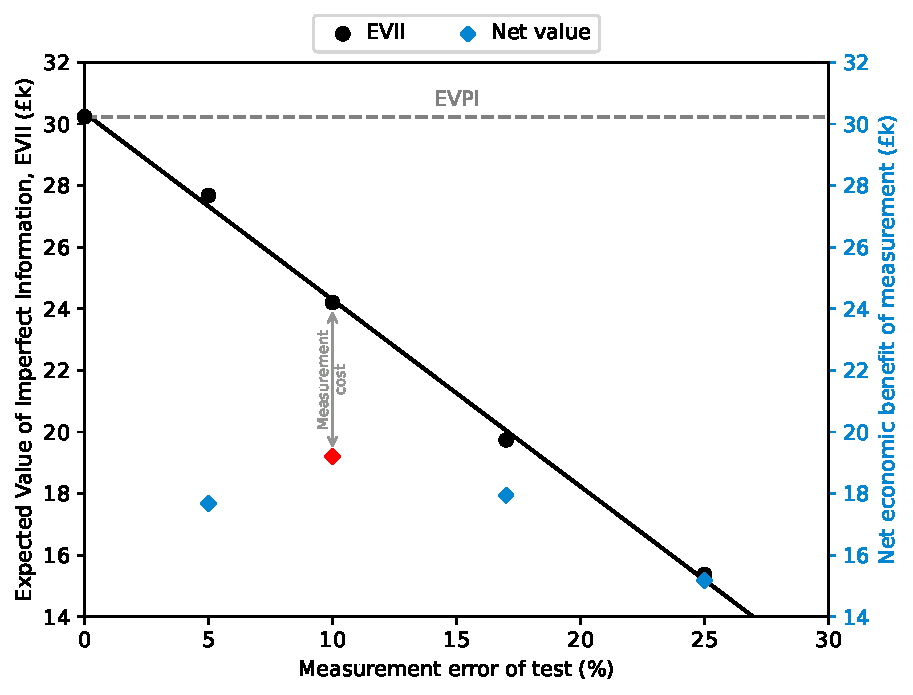
\includegraphics[width=0.8\linewidth]{GSHP_EVIIs.pdf}
    \vspace*{-0.2cm}
    \caption{\glsxtrlong{evii} (\glsxtrshort{evii}) and net economic benefit (\glsxtrshort{evii} minus measurement cost) of imprecise ground thermal conductivity measurements}
    \label{fig:GSHP-EVIIs}
\end{figure}


\newpage
%********************************** Conclusions **************************************
\section{Conclusions} \label{sec:demonstrations-conclusions}

This chapter demonstrated how \glsxtrshort{voi} can be used to quantify the benefit of data collection to support decision making in building energy systems, and as a decision support tool for evaluating data collection strategies. Three example decision problems covering the management, operation, and design of building energy systems were studied: heat pump maintenance scheduling, office ventilation scheduling, and ground source heat pump system design.

% ASHP maintenance
Installing smart meters in \glsxtrshort{ashp}s for dynamic maintenance scheduling was found to be a worthwhile investment. However, improvements in decision making provided were extremely limited, with perfect knowledge of heat pump condition leading to only a 0.06\% reduction in operational costs on average.
% Office ventilation
Occupancy monitoring systems enabled significant cost savings when scheduling ventilation to manage indoor air quality and infection risk in office spaces, reducing the total cost to the tenant by 10.2-16.4\%. Occupancy information was found to be more valuable in mid-sized offices and when infection is more prevalent, e.g. in the winter.
% GSHP design
When designing a \glsxtrshort{gshp} based heating system for a block of flats, ground thermal tests to reduce uncertainty in thermal conductivity were found to be beneficial to support system design. A Thermal Response Test (TRT) was determined to be the optimal data collection strategy, enabling net savings of £19k on the lifetime cost of the heating system.

In each example problem a different capability of the \glsxtrshort{voi} framework was demonstrated: the ability to simply and clearly represent and analyse decisions in complex engineering systems, the identification of system characteristics for which data collection is worthwhile, and the determination of optimal data collection strategies when trading-off measurement precision versus cost.

The examples in this chapter show that \glsxtrlong{voi} analysis gives a clear and principled methodology for addressing the current research gap of quantifying the benefit of data collection to support decision making in the building energy systems literature. It provides a route to rationalise data collection strategies and avoid resource wastage on low insight data as building digitisation progresses. However, these examples use significantly simplified models of how decisions are made in building energy systems, and don't got into much depth about how the uncertainty reduction that the data provides affects the decision making process.